\documentclass[msc,numbers]{formating/coppe}
\usepackage{amsmath,amssymb}    % simbolos macos providos pela AMS

\usepackage[linktocpage=true]{hyperref}
\usepackage{float}
\usepackage{subfig}

\usepackage[utf8]{inputenc}

\usepackage[english]{babel}
\usepackage{ae}
\usepackage{epigraph}

\usepackage{graphicx}

\usepackage{psfrag}
\usepackage{epsfig}
\usepackage{enumerate}
%
\usepackage{latexsym}
\usepackage{fancybox,fancyhdr}
\usepackage{xcolor}
\usepackage{pstricks}
\usepackage{pgf,tikz}
\usepackage{mathrsfs}
\usetikzlibrary{arrows}

\definecolor{xdxdff}{rgb}{0.49019607843137253,0.49019607843137253,1.}
\definecolor{ffffff}{rgb}{1.,1.,1.}
\definecolor{qqqqff}{rgb}{0.,0.,1.}
\definecolor{ffqqqq}{rgb}{1.,0.,0.}

%%%
%\usepackage[hypertex]{hyperref} %Make sure it comes last of your loaded packages
\hypersetup{
  verbose,
  plainpages=false,
  colorlinks=true,
  linkcolor=blue,
  anchorcolor=red,
  citecolor=green,
  filecolor=magenta,
  menucolor=red,
  urlcolor=blue
}

% Macros
\newtheorem{teorema}{Theorem}
\newtheorem{simulation}[teorema]{Simulacao}
\newtheorem{traj}[teorema]{Trajetoria}

\newcommand{\Appendix}{\par
  \setcounter{chapter}{0}
  \setcounter{section}{0}
  \setcounter{subsection}{0}
  \renewcommand{\chaptername}{\appendixname}
  \renewcommand{\thechapter}{\Alph{chapter}}
  \renewcommand{\thesection}{\Alph{chapter}.\arabic{section}}
  \renewcommand{\thesubsection}{\Alph{section}.\arabic{section}.\arabic{subsection}}
  \renewcommand{\theequation}{\Alph{chapter}{\arabic{equation}}}
}

\makelosymbols
\makeloabbreviations
\makeindex

\begin{document}
\selectlanguage{english}

\title{Mapeamento subaquático por Imaging Sonar}
\foreigntitle{Underwater Mapping Using Imaging Sonar}
\author{Eduardo}{Elael de Melo Soares}
\advisor{Prof.}{Ramon Romankevicius}{Costa}{D.Sc.}

\examiner{Prof.}{Ramon Romankevicius Costa}{D.Sc.}
\department{PEE} \date{01}{2016}
\keyword{Sonar} \keyword{Mapping}
\keyword{3D Reconstruction} \keyword{Underwater}
\maketitle
\frontmatter

\dedication{Mammy.}

\chapter*{Agradecimentos}
%%%
A Zeus,
\begin{foreignabstract}
%%%%%%%%%%%%%%%%%%%%%%%%%%%%%%%%%% ABSTRACT
This dissertation on 3D underwater simulation and mapping consists of two pieces
of software that is the main objective of the research, one for simulation and
another for mapping. A mapping system usually comes together with a localization
algorithm in what is called a SLAM (\textit{Simultaneous Localization and
Mapping}). SLAM is an active topic of research and has remarkable solutions
using laser scanners,
% http://www.frc.ri.cmu.edu/~jizhang03/Publications/RSS_2014.pdf
% http://www.frc.ri.cmu.edu/~jizhang03/Publications/IROS_2014.pdf
but most of the underwater SLAM is focused on 2D maps treating the environment
as a floor plant or as 2.5D maps on the seafloor.

The reason for the problematic of underwater mapping, and thus SLAM, takes part
in its sensor, i.e. sonars. Contrasting to laser-based systems used outside
water which are precise low-noise sensors.

The standard sensor, sonar, is composed of hydrophones which allows them to
measure sound in water. Therefore, enabling them to emit and receive sound
waves, resembling microphones and speakers. They are divided in passive sonars
and active sonars. Passive sonars can be applied to listen its surroundings,
interpreting the sounds by their spectrum.

Meanwhile, active sonars emit a beam of sound in order to perceive  and measure
the environment by the echo created. Active sonars are classified in two
important categories, profiling and imaging, based on its beam directional gain.

Profilings have a narrow pencil shaped beam  with an aperture of about $1.7$
degrees, i.e. the half power point. It is meant to have a similar response of a
laser scanner, despite working with sound waves. At last, they do not correlate
much, since they differ greatly on noise, response time and
spatial resolution.

Imaging sonars will be the focus of this work, they  employ a much wider beam
than profiling sonar. It is used to having around $3$ degrees angle of aperture
in the vertical direction, although keeping its same angular resolution on the
horizontal plane.
It does not have provide precise localization of the target, but a rather more
general information. Therefore, being able to infer the presence of objects
below or above its horizontal plane.
From this point of view, each beam gives broad  information about the region it
ensonifies. Thus, fusing multiple beams from different directions and angles,
containing overlapping areas,  is expected to provide a better outline of the
environment than just using isolated sonar responses.

Another classification, besides the one mentioned above, is the multi- or single
beam. Firing multiple beams at once gives a faster rate, not requiring waiting
for a response before redirecting the beam to its next angular position. When
working with multibeam sonar, its downside remains its market value. Contrasting
to the cheaper option, the single beam sonar, which will be further studied in
this thesis.
\end{foreignabstract}

\tableofcontents
\noindent
\mainmatter
%%%%%%%%%%%%%%%%%%%%%%%%%%%%%%%%%%%%%%%%%%
%%%%%%%%%%%%%%%%%%%%%%%%%%%%%%%%%%%%%%%%%%
\chapter{Introduction}

%% SrJ: add explanations about profiling vs. imaging: size of beam and
%% SrJ: implications (ambiguities)

Underwater mapping and simulation are dual processes, while the latter produce
sonar responses for a given environment, the former use these responses to infer
the surroundings. As such simulation is a flexible way of generating data with a
known ground truth to test a mapping algorithm. However, to archive a correct
underwater simulation algorithm, simplifying assumptions on sound physics
and environmental characteristics are necessary, as well as a definition of the
sonar type being modeled.
%SLAM 

Profilings and imaging sonars are two classes of sonars whose differences lie
in the aperture of their sound beams. Profiling sonars have a narrow sound beam
and they are considered the laser scanner analog for underwater mapping,
even though profilings still have much wider beam than lasers. The simplest
approaches to underwater 3D mapping focus on applying laser scanner techniques
to profiling sonars, e.g. point cloud reconstruction.
% % SrJ: they don't really "give more information". They cover more space per %
% SrJ: beam, but the information is more ambiguous
 On the other hand, imaging sonars are usually
cheaper and have a wider sound beam, covering more space at the expense of
having a more ambiguous response. Thus, the choice of using imaging
sonars for mapping comes with the challenge of overcoming its measurement's
uncertainty.
%and benefiting from its extra information is a win-win strategy, the .
% % SrJ: "a win-win strategy" means that there are two parties ... I only see
% one

%Mapping is subject to different interpretations,


% % SrJ: apart from poor wording, the following is off the point. What you
% really
% % SrJ: want to stress is that there are various map representations. There are
% % SrJ: SLAMs on dense 3D maps / 2.5D ! Not every SLAM is feature-based, and a
% % SrJ: lot of feature-based SLAMs can generate dense maps as a byproduct
Besides stipulating a sonar type, the meaning of mapping ought to be narrowed
down. It is possible to generically define mapping as the process of gathering
multiple sensor data to characterize the surroundings. However, how this
characterization might be represented is dependent on the application.

A SLAM (\textbf{S}imultaneous \textbf{L}ocalization \textbf{a}nd
\textbf{M}apping) system has no intrinsic need for a human readable map.
In such a system, it could be interesting to store the map information only
through its most representative features, but even for SLAM that is not always
the case. It is often implemented as a grid with empty/full cells or even as a
continuous map.

The mapping of underwater environments is not just a part of a SLAM system. It
has importance on its own, it can be used for humans to visualize things that
could not be seeing otherwise. If the map is to be seen by a human it should
store and merge information about the environment, so that it can be displayed
as a usual map, 3D or 2D depending on the case. This representation also guides
how the data could be stored, e.g. if it wants to show a surface, it can be
stored as an elevation map, or if one wants to see a 3D object it can be stored
as a point cloud, a 3D grid, a continuous map, etc.

\section{Purpose and Significance}
%\section{Motivation}

%% SrJ: OK, drop the whole "SLAM" thing. Really, just mention it briefly in the
%% SrJ: beginning of the introduction and STOP
%%
%% SrJ: you're not doing SLAM, and mapping is important. Period.

%% SrJ: AFAIK, you won't run your algorithm on any ESBR data .... I wouldn't
% % SrJ: mention it here
% The mapping of underwater environments is not just a part of a SLAM system. It
% might have importance on its own, it can be used for humans to visualize things
% that could not be seeing otherwise. 

In the ROSA (\textit{Robô para Operações de Stoplogs Alagados}) project,
developed by LEAD/COPPETEC for ESBR (Engenharia Sustentável do Brasil), one of
the goals is to make a reconstruction of the hydroelectric power plant turbine
entrance. It should spot any underwater debris that could block the lowering of
stoplogs\footnote{long rectangular timber beams stacked to block water
flow.} and cause delays or even accidents.
Interestingly, the stoplog setup has characteristics that make it appropriate
for sonar mapping. It has a lifting beam for inserting stoplogs into
water that can act as stable fixation point for any sonar structure and
provide a good means of localization. Well placed high-end sonars could probably
scan such a environment, but they are expensive.

Mechanical imaging sonar is a more affordable type of sonar, however it suffers
from imprecise measurements caused by its wide sound beam. This works aims to
provide a method to map an environment using imaging sonars. It extends a recent
developed continuous map technique (Hilbert maps~\cite{ramos2016hilbert}) by
applying it to sonar responses. It also implement a simulator with a trade-off
between having simplifying assumptions and being as complete as possible for
imaging sonars, justifying the choices based on first physical principles and
other advanced simulation techniques.


% 
% 
% %% SrJ: this is really ... out of context
% It is also a integral part ROV's, where it gives feedback to the operator for
% him to know where it is or/and what he is doing, especially because cameras do
% %% SrJ: I don't get that last sentence.
% not have a very useful range. And glaringly its automated counterpart (AUV's) as
% a requisite for SLAM.

\section{Review of the Literature}

********

1)Comment other simulators and what they miss (multipath or forwardlooking,
generally).
\citet{Coiras2009} - Simulation SAS
\citet{coiras2009gpu} - GPU based SAS

2)Cite first principles confusion on references (Intensity/RMS Acoustic
Pressure), Lambertian reflection, etc\ldots

3)Comment other mappings and what they miss (3D sonar or computability usually).
\\\\
******** 



\section{Objectives}

%% SrJ: try to be more bullet-pointy
%% SrJ: you already made your point about "that can be done in many ways" focus
%% SrJ: on what this thesis does.

% %, which technical details are based on Tritech's Micron sonar

The objectives of this work are the development of a simulator and a mapping
system for mechanical imaging sonars, thus being able to validate the hypothesis
that these sonars can be used for mapping.
The simulator will be able to receive a description of a general environment and calculate the expected response of a high-frequency imaging sonar. Its output
shall exhibit common sonar features as multipath effects, noise and beamwidth
uncertainty. The response will be presented as polar plot similar to those used
by real sonars.

The mapping system will receive sonar measurements, typically the simulator's
output, and generate a Hilbert map representation of the continuous occupancy
map, by apply a simple embedding of sonar response method envisioned by the
author.
The map has to match to the simulator ground truth avoiding inconsistencies
caused by the sonar's wide beam. The Hilbert map representation is, technically,
just a vector that encodes 3D occupancy maps, however the information of this 3D
map will be displayed as 2D cross-sections for better readability.


% The general objective is to map an underwater environment.
% But that can be done in many ways, for this thesis the main goal is to implement
% optimization of the visible surface based on the expected response of a
% sonar beam in a given direction and fuse multiple views using binary bayesian
% filters. 
% 
% The output of the whole process will be a 3D human-redable map of the scanned
% environemnt. The optimization step might, also, supply information about the
% surface material, specifically its reflectance. A technique based on previously
% articles.
% 
%  Fuse all the data on a octree structure using a robotic framework,
% named ROCK, and implement a visualization for the reconstruct underwater map.
% The data source shall be a imaging sonar mounted on a pan-tilt unit, so to
% provide the sonar extra degrees of freedom.

%  But to get there it is important to describe some facts first.
%  
% As stated before, profiling sonar try to mimic laser scanner, but using sound.
% So most of the approaches on 3D underwater SLAM focus on applying laser scanner
% techniques to profiling sonars, e.g. point cloud reconstruction. On the other
% hand, imaging sonars are usually cheaper and gives more information per sound
% beam. So having the possibility of using imaging sonar and benefiting from its
% extra information is a win-win strategy.
% 
% Besides the definition of the sonar, one should carefully look into the meaning
% of mapping, because, it can be interpreted in different ways, depending on the
% context.
% Taking what they all have in common, it is possible to generically define
% mapping as being the process of received environmental data to characterize
% the surroundings. In the understanding of characterization is where the
% difference lays, how the environs are going to be represented is dependent on
% the application.
% 
% On a SLAM system there is no intrinsic need for a human readable map. In such a
% system, it may be more interesting to store the map information, the
% \"characterization\", only through its most representative features, if that is
% what matters for the localization procedure.
% 
% Still, if the map is to be seen by a human it should store more information
% about the environment, so that it can be displayed as a usual map, 3D or 2D
% depending on the case. This representation also guides how the data could be
% stored, e.g. if it wants to show a surface, it can be stored as an elevation map,
% or if one wants to see a 3D object it can be stored as a point cloud.
% 
% Using de aforementioned ideas, the main goal of the thesis reported here is to
% implement state-of-the-art techniques for mapping, using binary bayesian
% filters. Fuse all the data on a octree structure using a robotic framework,
% named ROCK, and implement a visualization for the reconstruct underwater map.
% The data source shall be a imaging sonar mounted on a pan-tilt unit, so to
% provide the sonar extra degrees of freedom.
% 
% Optimization of the visible surface for based on the expected response of a
% sonar beam in a given direction will also be attempted. It might supply
% information about the surface material, specifically its reflectance. A
% technique based on previously articles.



\section{Methodology}
%\section{Metodology and Expected Results}
%But to get there it is important to describe some facts first.
 


% Using de aforementioned ideas, the main goal of the thesis reported here is to
% implement state-of-the-art techniques for mapping, using binary bayesian
% filters. Fuse all the data on a octree structure using a robotic framework,
% named ROCK, and implement a visualization for the reconstruct underwater map.
% The data source shall be a imaging sonar mounted on a pan-tilt unit, so to
% provide the sonar extra degrees of freedom.
% 
% Optimization of the visible surface for based on the expected response of a
% sonar beam in a given direction will also be attempted. It might supply
% information about the surface material, specifically its reflectance. A
% technique based on previously articles.


This work is divided into two parts.

The sonar model definition starts with a compilation on the description of
sonar, physical properties of sound waves in water, reflection, sonar
directional gain and sources of noise. Those are used to select a simulation
technique and model two different environment, a simple and a complex
structure, one to feed to the mapping algorithm and another to explore more
advanced acoustic features, e.g. multipath, directional gain. The simulation
results for both environments are then analyzed for those typical sonar
features.

The second part is related to mapping. An introductory chapter presents
the mathematical concepts used, followed by another with discussions on the
difficulties of 3D reconstruction and its methods. The latter includes description
of the most common and standard state-of-the-art techniques, with comments on
some alternative works, and deeper details of Hilbert maps. Hilbert maps
implementation and results, for one of the simulated environments, are
displayed at the end of the chapter.

% The second branch deal with the map filling over a discretized space, based on
% a Binary Bayesian Filter implementation. That is the standard state-of-the-art
% technology for mapping \cite{thrunprob}.


% The second branch deal with the map filling, basically the Binary Bayesian
% Filter implementation. A review on Bayesian Filtering is scheduled before the
% coding writing to be done on the robotics framework, ROCK. The implementation
% will make use of the Octotree data structure, through the Octomap library, to
% store the map.

% The integration of the sonar model with the Bayesian Filter give the means to
% process sonar data. So data acquired on the LNDC/UFRJ tank (Laboratório de
% Ensaios Não Destrutivos, Corrosão e Soldagem - which loosely translated means
% Non-Destructive Testing, Corrosion and Welding Laboratory) and on the Jirau
% Power Plant, by means of the ROSA/COPPETEC project, will be processed and
% compared to the tank and power plant entry layout, respectively.
%  
% In a more complex endeavor, which is the third branch, a theoretical derivation
% for the optimization of 2D surfaces embed on 3D environments will take place.
% It uses the sonar response as expectation and, instead of having a fixed
% relation between the measured environment and the sonar response, aim to better
% infer the underlying geometry of the surrounds and also retrieve some
% information about the material's reflectivity properties.
% This optimization algorithm will then be integrated into the Bayesian Filter. The
% same data processed by the combination ``Filter + Sonar Model'' shall now be
% processed by ``Filter + Optimization''.
%  
% Based on the literature, even with not much similar works, the reconstruction
% with \textit{a priori} sonar model will probably experience problems when
% reconstructing corners, shallow angle surfaces, very complex (intense multipath)
% or on highly noise environments. For the optimization, it shall encounter
% similar issues, but a less accentuated shallow angle quality degradation and an
% overall less blurry reconstruction.

\section{Work Structure}

\textbf{Chapter 1}\quad Motivation and general description of the thesis.
\\
\textbf{Chapter 2}\quad Description of sonar models and their working
principle. Development of simulation logic from acoustics. Review of
simulations techniques on the literature. Implementation and results of a
simulator based on a ray theory algorithm.
\\
\textbf{Chapter 3}\quad Presentation of the mathematical structure necessary for
understanding Hilbert Maps.
\\
\textbf{Chapter 4}\quad Review of mapping techniques on the literature.
Detailed description of Hilbert Maps and a proposal of sonar response embbeding.
Implementation and results for a box-like environment, from a simulation of
chapter 2.
\\
\textbf{Chapter 5}\quad Comparison between simulation ground truth and
reconstructed environment. Suggestion of next steps to improve both simulation
and mapping.
% 
% ********
% 
% 1) First principles -> Ray Theory (other techniques along the way)
% 
% 2) Enronments and Materials
% 
% 3) Simulation and Results
% 
% 4) Math to Mapping
% 
% 5) Mapping concept
% 
% 6) Mapping implementation and results
% 
% 7) Conclusion / Comparison
% \\\\
% ********

\chapter{Sonar Simulation}

\epigraph{If you cause your ship to stop, and place the head of a long tube in
the water and place the outer extremity\\ in your ear, you will hear ships at a
great distance from you.}{\textit{Leonardo Da Vinci}, 1490}


The ideia behind simulation is to have a flexible environment where the system
(e.g. sonar, reconstruction model) can be tested on a variety of conditions
and the ground truth is well known. It is a mature and wide spread
mechanism for development of new sonar technologies \cite{Etter2013}.

This chapter start with a small revision on the physics and history behind
sonars, explore the existing technologies and models. Then describes the
envisioned environment properties. And finish with a more detailed view of
the simulation technique used.

\section{Sonar}

Throughout this thesis only one type of sonar is considered, the mechanical
imaging active sonar\ref{ss:avaible_models}. Sonars have a common underlying
principle of operation, but vary greatly on aplication and hardware constituition.

Sonars are, in some sense, the acoustic analog of a camera. They use sound,
instead of light, to capture information about the environment. So, to better
undersand \textit{how} they operate and \textit{what} are they used for, it is
important to have a clear concept of sound.

\subsection{Physics of Sound}

The phenomenon that humans percieve as sound is a pressure wave that amplitude
excess the mean pressure of the medium \cite{FEYNMAN}. It can me referred to as
\textit{compressional} or \textit{longitudinal} waves, contrasting with
\textit{transversal waves}. The difference between these two kinds of waves
relies on the direction of the movement of the particles, being parallel or
perpendicular to the propagation of the wave, respectively\cite{BRUNEAU}.

On the particular, but usefull, conditions of low energy
phenomena\cite{Lefebvre} (with some other suitable requirements\footnote{A
perfect simple fluid in an initial state of stationary homogeneous equilibrium})
the pressure pertubation wave can be described as the \textit{D'Alembert
equation}:
 
\begin{equation}\label{eq:lambert}
\nabla^2 \Phi - \frac{1}{c^2_0}\frac{\partial^2}{\partial t^2} \Phi = 0
\end{equation}

Where $\Phi$ is the velocity potencial, a scalar field that helps describing the
sound propagation. Its relation to sound pressure is:

\[ p =  -\rho \frac{\partial}{\partial t}\Phi \]

Which can be directly described as:

\begin{equation} \label{eq:wave}
\nabla^2 p - \frac{1}{c^2_0}\frac{\partial^2}{\partial t^2} p = 0
\end{equation} 
 
Where $p$ is the pressure deviation from the mediums, $\rho$ the density, $c_0$
is the local sound speed and $\nabla^2$ stands for the Laplace operator. These equations are
only valid in free space (no source), but discrete variations of the medium are
treated as boundary conditions, giving origin to reflection and refraction.

Besides pressure, sound has another important derived property: intensity. Much
like the case of electromagnetic waves, sound intensity (or acoustic intensity)
measures the mean value of the sound energy flux (i.e. energy rate
per area):

\begin{equation}\label{eq:intensity_mean}
\vec{I} = \overline{p\vec{v}}
\end{equation}

Where $\vec{I}$ represents the \textit{acoustic intensity} vector, $\vec{v}$ the
\textit{acoustic velocity} (i.e. the velocity of a particle in the medium) and the
overline the mean over some time period. The \textit{acoustic velocity} can also
be derived from the velocity potencial $\Phi$ as:

\[ \vec{v} = \nabla \Phi\]

When considering a wave far from its source, solutions to the equation
\ref{eq:wave} give rise to a \textit{plane wave}( where the coherent wave front
propagate in a plane). It makes clear the relationship between $\vec{v}$ and
$p$:

\[ \vec{v} = \frac{p}{\rho c_0} \vec{n_0} \]

Where $\vec{n_0}$ is the unit normal vector to the wavefront. Pluging it back to
equation \ref{eq:intensity_mean}:

\begin{equation}\label{eq:intensity_pressure}
\vec{I} = \tfrac{1}{\rho c_0} \overline{p^2} \vec{n_0}
\end{equation}

This equation shows the proportionality between the \textit{acoustic
intensity} and the mean squared of the pressure. The inverse of the
proportionality constant $\rho c_0$ is called the \textit{characteristic
impendace} because it measures the degree of ``resistense to propagation'' of
the medium.

%By means of the same reasoning about the physical properties

 %(perpendicular to the direction of propagation)

Because the acoustic intensity (and related quantities) varies orders of
magnitude while propagating, it is commom to quantify it on a logarithmic scale,
specifically \textit{decibels} (dB)\cite{LURTON}:

\begin{equation}\label{eq:dB}
I_{dB} = 10~\log_{10}\left(\frac{I}{I_0}\right)
\end{equation} 

Here $I_{dB}$ is the intensity measured in \textit{decibels}, $I$ the intensity
value and $I_0$ a reference intensity values, usually defined somewhere near the
source. In the case of reflected/refracted wave, $I_0$ may also refere to
the intensity of the incoming wave. A direct relation between the magnitude of
intensity and pressure is found by applying equation \ref{eq:intensity_pressure}
on equation\ref{eq:dB}:

\begin{equation}\label{eq:dB}
I_{dB} = 20~\log_{10}\left(\frac{p_{\text{rms}}}{p_0}\right)
\end{equation}

Where $p_{\text{rms}}$ is the \textit{rms} (Root mean squared) value of the
wave's pressure ({\small $\sqrt{\text{\tiny \(\overline{p^2}\)}}$}) and $p_0$ is
a pressure value of reference, for underwater acoustics this value is the
microPascal (\(p_0 = 1~\mu\text{Pa} \))\cite{LURTON}.


\subsection{Sonar Principle of Operation}

The name Sonar (\textit{\underline{So}und \underline{N}avigation \underline{A}nd
\underline{R}anging}) was originally conceived for the tecnique that uses
acoustic waves on water for navigation, communication and detection, but
nowadays it is also used for the equipament that generate/receive these
sound waves.

The history is considered to have started on the year of 1490 through the
statemnt of Leonardo Da Vinci contained on the epigraph at the begining of this
chapter\cite{fahy1998fundamentals}. But that was birth of \textit{passive
sonar}'s technology, where the objetive is to listen (receive and process sound
waves) the noise from ships, animals and other objects in an attempt detect and
reconize its origin.

\subsubsection{Active Sonar}

The concept of an \textit{active sonar}, one that emits a sound wave and detects
its return (as in figure \ref{fig:sonar_principle}), is much more recent. The
loss of the \textit{HMS Titanic} to a collision with an iceberg during its first
voyage on April 15 of 1912 \cite{histsonar} fostered the development of a sonar
to detect objects kilometers away. Also, during World War I,
Allied shipping losses to U-boat attacks further stimulated advances on tecniques for
unconvering of submerged enemies.

\begin{figure}
	\centering
		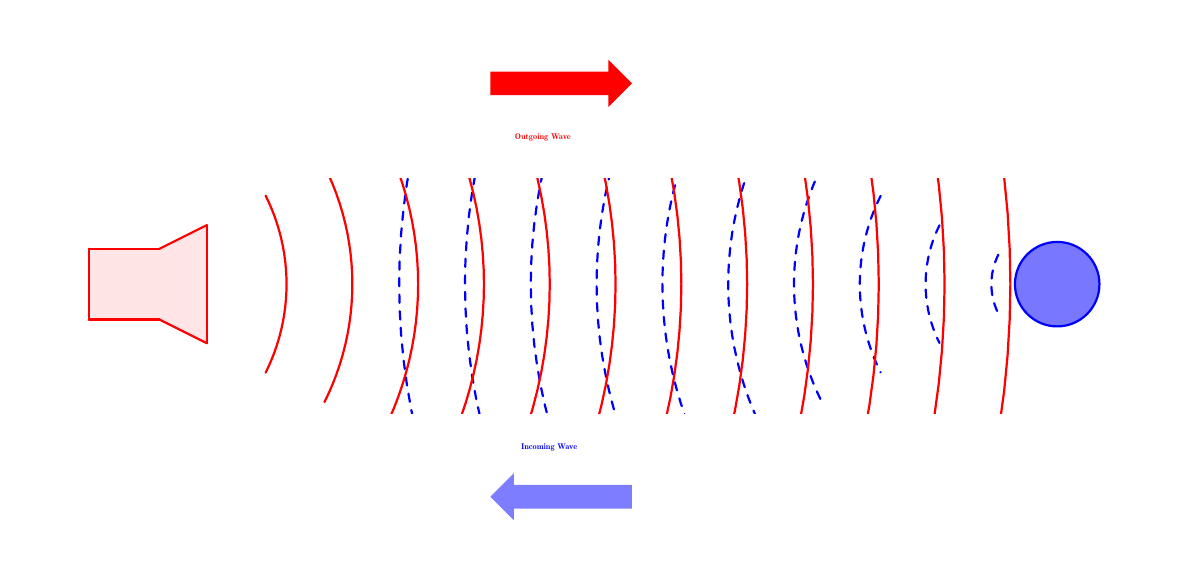
\begin{tikzpicture}[thick,scale=0.3, every node/.style={transform shape},line
	cap=round,line join=round,>=triangle 45,x=1.0cm,y=1.0cm] \clip(2.4174670085420336,-13.987437987397216) rectangle (50.355233369869445,8.357537118695749);
	\fill[color=ffqqqq,fill=ffqqqq,fill opacity=0.1] (5.,-4.) -- (5.,-1.) -- (8.,-1.) -- (10.,0.) -- (10.,-5.) -- (8.,-4.) -- cycle;
	\draw [color=qqqqff,fill=qqqqff,fill opacity=0.53] (46.,-2.5) circle (1.7879362227931317cm);
	\draw [color=ffqqqq] (5.,-4.)-- (5.,-1.);
	\draw [color=ffqqqq] (5.,-1.)-- (8.,-1.);
	\draw [color=ffqqqq] (8.,-1.)-- (10.,0.);
	\draw [color=ffqqqq] (10.,0.)-- (10.,-5.);
	\draw [color=ffqqqq] (10.,-5.)-- (8.,-4.);
	\draw [color=ffqqqq] (8.,-4.)-- (5.,-4.);
	\draw [shift={(5.,-2.5)},color=ffqqqq]  plot[domain=-0.46364760900080615:0.4636476090008061,variable=\t]({1.*8.375892603043697*cos(\t r)+0.*8.375892603043697*sin(\t r)},{0.*8.375892603043697*cos(\t r)+1.*8.375892603043697*sin(\t r)});
	\draw [color=ffffff] (4.,2.)-- (50.,2.);
	\draw [color=ffffff] (50.,2.)-- (50.,10.);
	\draw [color=ffffff] (50.,10.)-- (4.,10.);
	\draw [color=ffffff] (4.,10.)-- (4.,2.);
	\draw [color=ffffff] (44.,-8.)-- (4.,-8.);
	\draw [color=ffffff] (4.,-8.)-- (4.,-16.);
	\draw [color=ffffff] (4.,-16.)-- (42.20321483552447,-16.390821937761867);
	\draw [color=ffffff] (42.20321483552447,-16.390821937761867)-- (44.,-8.);
	\draw [shift={(46.,-2.5)},dash pattern=on 3pt off 3pt,color=qqqqff]  plot[domain=2.6779450445889874:3.6052402625905975,variable=\t]({1.*2.785722659294224*cos(\t r)+0.*2.785722659294224*sin(\t r)},{0.*2.785722659294224*cos(\t r)+1.*2.785722659294224*sin(\t r)});
	\draw [shift={(46.,-2.5)},dash pattern=on 3pt off 3pt,color=qqqqff]  plot[domain=2.6779450445889874:3.6052402625905993,variable=\t]({1.*5.571445318588448*cos(\t r)+0.*5.571445318588448*sin(\t r)},{0.*5.571445318588448*cos(\t r)+1.*5.571445318588448*sin(\t r)});
	\draw [shift={(46.,-2.5)},dash pattern=on 3pt off 3pt,color=qqqqff]  plot[domain=2.677945044588987:3.6052402625905997,variable=\t]({1.*8.357167977882664*cos(\t r)+0.*8.357167977882664*sin(\t r)},{0.*8.357167977882664*cos(\t r)+1.*8.357167977882664*sin(\t r)});
	\draw [shift={(46.,-2.5)},dash pattern=on 3pt off 3pt,color=qqqqff]  plot[domain=2.677945044588987:3.6052402625905993,variable=\t]({1.*11.142890637176889*cos(\t r)+0.*11.142890637176889*sin(\t r)},{0.*11.142890637176889*cos(\t r)+1.*11.142890637176889*sin(\t r)});
	\draw [shift={(46.,-2.5)},dash pattern=on 3pt off 3pt,color=qqqqff]  plot[domain=2.677945044588987:3.605240262590599,variable=\t]({1.*13.928613296471113*cos(\t r)+0.*13.928613296471113*sin(\t r)},{0.*13.928613296471113*cos(\t r)+1.*13.928613296471113*sin(\t r)});
	\draw [shift={(46.,-2.5)},dash pattern=on 3pt off 3pt,color=qqqqff]  plot[domain=2.677945044588987:3.6052402625905993,variable=\t]({1.*16.714335955765335*cos(\t r)+0.*16.714335955765335*sin(\t r)},{0.*16.714335955765335*cos(\t r)+1.*16.714335955765335*sin(\t r)});
	\draw [shift={(46.,-2.5)},dash pattern=on 3pt off 3pt,color=qqqqff]  plot[domain=2.677945044588987:3.6052402625905993,variable=\t]({1.*19.500058615059555*cos(\t r)+0.*19.500058615059555*sin(\t r)},{0.*19.500058615059555*cos(\t r)+1.*19.500058615059555*sin(\t r)});
	\draw [shift={(46.,-2.5)},dash pattern=on 3pt off 3pt,color=qqqqff]  plot[domain=2.677945044588987:3.6052402625905993,variable=\t]({1.*22.285781274353777*cos(\t r)+0.*22.285781274353777*sin(\t r)},{0.*22.285781274353777*cos(\t r)+1.*22.285781274353777*sin(\t r)});
	\draw [shift={(46.,-2.5)},dash pattern=on 3pt off 3pt,color=qqqqff]  plot[domain=2.677945044588987:3.605240262590599,variable=\t]({1.*25.071503933648003*cos(\t r)+0.*25.071503933648003*sin(\t r)},{0.*25.071503933648003*cos(\t r)+1.*25.071503933648003*sin(\t r)});
	\draw [shift={(46.,-2.5)},dash pattern=on 3pt off 3pt,color=qqqqff]  plot[domain=2.677945044588987:3.6052402625905993,variable=\t]({1.*27.857226592942222*cos(\t r)+0.*27.857226592942222*sin(\t r)},{0.*27.857226592942222*cos(\t r)+1.*27.857226592942222*sin(\t r)});
	\draw [shift={(5.,-2.5)},color=ffqqqq]  plot[domain=-0.46364760900080615:0.4636476090008061,variable=\t]({1.*11.16161526233792*cos(\t r)+0.*11.16161526233792*sin(\t r)},{0.*11.16161526233792*cos(\t r)+1.*11.16161526233792*sin(\t r)});
	\draw [shift={(5.,-2.5)},color=ffqqqq]  plot[domain=-0.46364760900080615:0.4636476090008061,variable=\t]({1.*13.947337921632139*cos(\t r)+0.*13.947337921632139*sin(\t r)},{0.*13.947337921632139*cos(\t r)+1.*13.947337921632139*sin(\t r)});
	\draw [shift={(5.,-2.5)},color=ffqqqq]  plot[domain=-0.46364760900080615:0.4636476090008061,variable=\t]({1.*16.733060580926363*cos(\t r)+0.*16.733060580926363*sin(\t r)},{0.*16.733060580926363*cos(\t r)+1.*16.733060580926363*sin(\t r)});
	\draw [shift={(5.,-2.5)},color=ffqqqq]  plot[domain=-0.46364760900080615:0.4636476090008061,variable=\t]({1.*19.51878324022059*cos(\t r)+0.*19.51878324022059*sin(\t r)},{0.*19.51878324022059*cos(\t r)+1.*19.51878324022059*sin(\t r)});
	\draw [shift={(5.,-2.5)},color=ffqqqq]  plot[domain=-0.46364760900080615:0.4636476090008061,variable=\t]({1.*22.304505899514808*cos(\t r)+0.*22.304505899514808*sin(\t r)},{0.*22.304505899514808*cos(\t r)+1.*22.304505899514808*sin(\t r)});
	\draw [shift={(5.,-2.5)},color=ffqqqq]  plot[domain=-0.46364760900080615:0.4636476090008061,variable=\t]({1.*25.090228558809027*cos(\t r)+0.*25.090228558809027*sin(\t r)},{0.*25.090228558809027*cos(\t r)+1.*25.090228558809027*sin(\t r)});
	\draw [shift={(5.,-2.5)},color=ffqqqq]  plot[domain=-0.46364760900080615:0.4636476090008061,variable=\t]({1.*27.875951218103253*cos(\t r)+0.*27.875951218103253*sin(\t r)},{0.*27.875951218103253*cos(\t r)+1.*27.875951218103253*sin(\t r)});
	\draw [shift={(5.,-2.5)},color=ffqqqq]  plot[domain=-0.46364760900080615:0.4636476090008061,variable=\t]({1.*30.661673877397476*cos(\t r)+0.*30.661673877397476*sin(\t r)},{0.*30.661673877397476*cos(\t r)+1.*30.661673877397476*sin(\t r)});
	\draw [shift={(5.,-2.5)},color=ffqqqq]  plot[domain=-0.46364760900080615:0.4636476090008061,variable=\t]({1.*33.4473965366917*cos(\t r)+0.*33.4473965366917*sin(\t r)},{0.*33.4473965366917*cos(\t r)+1.*33.4473965366917*sin(\t r)});
	\draw [shift={(5.,-2.5)},color=ffqqqq]  plot[domain=-0.46364760900080615:0.4636476090008061,variable=\t]({1.*36.23311919598592*cos(\t r)+0.*36.23311919598592*sin(\t r)},{0.*36.23311919598592*cos(\t r)+1.*36.23311919598592*sin(\t r)});
	\draw [shift={(5.,-2.5)},color=ffqqqq]  plot[domain=-0.46364760900080615:0.4636476090008061,variable=\t]({1.*39.018841855280144*cos(\t r)+0.*39.018841855280144*sin(\t r)},{0.*39.018841855280144*cos(\t r)+1.*39.018841855280144*sin(\t r)});
	\draw [color=ffqqqq] (24.,5.5)-- (27.,5.5);
	\draw [color=ffqqqq] (27.,5.5)-- (27.,5.);
	\draw [color=ffqqqq] (27.,5.)-- (27.5,5.5);
	\draw [color=ffqqqq] (27.5,5.5)-- (28.,6.);
	\draw [color=ffqqqq] (28.,6.)-- (27.5,6.5);
	\draw [color=ffqqqq] (27.5,6.5)-- (27.,7.);
	\draw [color=ffqqqq] (27.,7.)-- (27.,6.5);
	\draw [color=ffqqqq] (27.,6.5)-- (22.,6.5);
	\draw [color=ffqqqq] (22.,6.5)-- (22.,5.5);
	\draw [color=ffqqqq] (22.,5.5)-- (24.,5.5);
	\draw [color=xdxdff] (26.,-12.)-- (23.,-12.);
	\draw [color=xdxdff] (23.,-12.)-- (23.,-12.5);
	\draw [color=xdxdff] (23.,-12.5)-- (22.5,-12.);
	\draw [color=xdxdff] (22.5,-12.)-- (22.,-11.5);
	\draw [color=xdxdff] (22.,-11.5)-- (22.5,-11.);
	\draw [color=xdxdff] (22.5,-11.)-- (23.,-10.5);
	\draw [color=xdxdff] (23.,-10.5)-- (23.,-11.);
	\draw [color=xdxdff] (23.,-11.)-- (28.,-11.);
	\draw [color=xdxdff] (28.,-11.)-- (28.,-12.);
	\draw [color=xdxdff] (28.,-12.)-- (26.,-12.);
	\fill[color=ffffff,fill=ffffff,fill opacity=1.0] (4.,2.) -- (50.,2.) -- (50.,10.) -- (4.,10.) -- cycle;
	\fill[color=ffffff,fill=ffffff,fill opacity=1.0] (44.,-8.) -- (4.,-8.) -- (4.,-16.) -- (42.20321483552447,-16.390821937761867) -- cycle;
	\fill[color=ffqqqq,fill=ffqqqq,fill opacity=1.0] (24.,5.5) -- (27.,5.5) -- (27.,5.) -- (27.5,5.5) -- (28.,6.) -- (27.5,6.5) -- (27.,7.) -- (27.,6.5) -- (22.,6.5) -- (22.,5.5) -- cycle;
	\fill[color=xdxdff,fill=xdxdff,fill opacity=1.0] (26.,-12.) -- (23.,-12.) -- (23.,-12.5) -- (22.5,-12.) -- (22.,-11.5) -- (22.5,-11.) -- (23.,-10.5) -- (23.,-11.) -- (28.,-11.) -- (28.,-12.) -- cycle;
	\draw [color=ffqqqq](22.911186909624416,4.005463478846246) node[anchor=north west] {\textbf{Outgoing Wave}};
	\draw [color=qqqqff](23.17101220155573,-9.115713763685088) node[anchor=north west] {\textbf{Incoming Wave}};
	\end{tikzpicture}

	\caption{Depiction of the working principle of a \textit{active sonar}. The
	red speaker-like represented object represents the transducer, responsible for
	emiting and receiving the acoustic wave.}
	\label{fig:sonar_principle}
\end{figure}

Active sonars are ranging sensor and the way they infer distance is by measuring
the time between the emission and reception of a acoustic pulse (a time bounded
sound wave) like on \ref{fig:sonar_principle}. To be able to know space from the
delay, the mean sound speed of the medium throughout the path traveled by the
pulse has to be known\cite{LURTON}:

\begin{equation}
D = \frac{c_0 \Delta t}{2}
\label{eq:delaytodistance}
\end{equation}


Where $D$ is the distance between the source and the target, $c_0$ the mean
sound speed, $\Delta t$ the delay between pulse emission and reception, and
the denominator $2$ is there because the time is measuring a two way trip of
the sound. When the sound wave travel long distances in the ocean, the sound
speed can vary greatly, so special care should be taken\cite{Etter2013} (like
stratify the environment by same sound speed layers).

\subsubsection{Multipath}

Besides sound speed variation, another common issue is \textit{multipath}. The
moment a sound wave encounters an interface (e.g. sea floor, water surface or an
obstacle) it does not bounces back to the source, it also undergoes refraction
and reflection in other directions. Thus an eco that traveled a longer path may
also arrive, causing a naive application of equation \ref{eq:delaytodistance} to
predict the presence of an object further way (figure \ref{fig:multipath}). For
low-frequency sable signals, the contribution of all multipaths creates a
interference pattern\cite{LURTON}, a fact that will not be explored. 

\begin{figure}
	\centering
	\begin{tikzpicture}[thick,scale=0.25,line
cap=round,line join=round,>=triangle 45,x=1.0cm,y=1.0cm] \clip(1.6275066818196025,-8.839384430530606) rectangle (51.76470824776055,15.208548396032874);
\clip(3.1041672991448848,-7.273988531661666) rectangle (49.67584843845491,14.87093936751221);
\begin{scriptsize}
\draw [color=xdxdff] (44.21347454534831,-2.428987771071691)-- ++(-2.5pt,-2.5pt) -- ++(5.0pt,5.0pt) ++(-5.0pt,0) -- ++(5.0pt,-5.0pt);
\draw[color=xdxdff] (43.541104898818894,-3.402366846586503) node {$T$};
\draw [color=dcrutc] (42.93049589992042,11.940544124335187)-- ++(-2.0pt,-2.0pt) -- ++(4.0pt,4.0pt) ++(-4.0pt,0) -- ++(4.0pt,-4.0pt);
\draw[color=dcrutc] (42.45630268754179,10.625247954410463) node {$S$};
\draw[color=dcrutc] (-15.15043542855254,31.53574575109661) node {$s$};
\draw[color=xdxdff] (-14.477109918104684,30.37612959421419) node {$r$};
\end{scriptsize}
\fill[color=ffqqqq,fill=ffqqqq,fill opacity=0.1] (5.,-4.) -- (5.,-1.) -- (8.,-1.) -- (10.,0.) -- (10.,-5.) -- (8.,-4.) -- cycle;
\draw [dotted,color=dcrutc] (5.,-2.5) circle (40.586350338762315cm);
\draw [dash pattern=on 3pt off 3pt,color=dcrutc] (44.59640537748493,12.574773620869905) circle (1.7825571147199057cm);
\draw [dotted,color=xdxdff] (5.,-2.5) circle (39.21353884381436cm);
\draw [color=ffqqqq] (5.,-4.)-- (5.,-1.);
\draw [color=ffqqqq] (5.,-1.)-- (8.,-1.);
\draw [color=ffqqqq] (8.,-1.)-- (10.,0.);
\draw [color=ffqqqq] (10.,0.)-- (10.,-5.);
\draw [color=ffqqqq] (10.,-5.)-- (8.,-4.);
\draw [color=ffqqqq] (8.,-4.)-- (5.,-4.);
\draw [color=qqqqff,fill=qqqqff,fill opacity=0.53] (46.,-2.5) circle (1.7879362227931317cm);
\draw [->,line width=1.6pt,dash pattern=on 6pt off 6pt,color=dcrutc] (24.7,5.) -- (42.93049589992042,11.940544124335187);
\draw [->] (10.,-0.5964467005076142) -- (24.7,5.);
\draw [->] (24.7,5.) -- (44.21347454534831,-2.428987771071691);
\draw [->] (44.21347454534831,-2.428987771071691) -- (10.,-2.4909454301421077);
\draw [line width=2.pt] (20.,5.)-- (35.,5.);
\end{tikzpicture}
	\caption{Visualization of a multipath for a high frequency short pulse (much
	smaller then delay times). Black vectors show the path taken by the sound
	wave. Red dashed vector show the calculated distance by equation
	\ref{eq:delaytodistance}.}
	\label{fig:multipath}
\end{figure}

\subsubsection{Sonar Resolution and Chirp Pulses}

The minimum distance (or eco delay) that can be resolved by the sonar depends on
the type of the pulse emitted (figure \ref{fig:chirpresolution}). There are two
main types of pulse:
\textit{single frequency} and \textit{chirp}\cite{chirp,gaussianchirp}. Some
sonars use dual frequency to overcome the trade-off between reach and resolution, given that low-frequency have a longer
range and high-frequency a better resolution.

For single frequency sonar the limit resolution ($\delta D$) depends directly on
the pulse length ($\Delta\text{L}$):

\[ \delta D = \frac{c_0~\Delta\text{L}}{2} \] 

However, that limitation can be overcome by the use of pulse compression (a
cross-correlation filter like matched filters). In this case, a linear varying
frequency signal (chirp), or similar multifrequency systems, have its resolution
related to the bandwidth ($\Delta \text{BW}$):

\[ \delta D = \frac{c_0}{2~\Delta \text{BW}} \]

\begin{figure}
	\centering
	% Need GNUPLOT installed
% also include the command:
% pdflatex --shell-escape --enable-write18
\begin{tikzpicture}[thick,scale=0.25, line
cap=round,line join=round,>=triangle 45,x=1.0cm,y=1.0cm] \clip(3.293642526630789,-8.675027400644247) rectangle (53.399160386607996,4.134242296170057);\draw[color=qqqqff, smooth,samples=400,domain=-18.1:18.1]
plot[parametric]
function{10.0+t+18.1,-2.512006409518489+1.7*2.718281828**((-t**(2.0))/2.0)*cos((18.1*t**(2.0)/2.0))};
\draw[color=qqwuqq, smooth,samples=400,domain=-20.4:20.4] plot[parametric]
function{10.0+t+20.4,-2.512006409518489+1.7*2.718281828**((-t**(2.0))/2.0)*cos((18.1*t**(2.0)/2.0))};
\fill[color=ffqqqq,fill=ffqqqq,fill opacity=0.1] (5.,-4.) -- (5.,-1.) -- (8.,-1.) -- (10.,0.) -- (10.,-5.) -- (8.,-4.) -- cycle;
\draw [color=qqqqff,fill=qqqqff,fill opacity=1.0] (46.199994390887134,-2.512006409518489) circle (1.788cm);
\draw [color=qqwuqq,fill=qqwuqq,fill opacity=1.0]
(50.79999363285944,-2.512006409518489) circle (1.788cm); \draw [color=ffqqqq]
(5.,-4.)-- (5.,-1.); \draw [color=ffqqqq] (5.,-1.)-- (8.,-1.); \draw
[color=ffqqqq] (8.,-1.)-- (10.,0.); \draw [color=ffqqqq] (10.,0.)-- (10.,-5.);
\draw [color=ffqqqq] (10.,-5.)-- (8.,-4.); \draw [color=ffqqqq] (8.,-4.)--
(5.,-4.);
\draw (25.872236701327112,2.1879575012477424) node[anchor=north west, scale =
0.7] {Resolution}; \draw (28.,0.2)-- (28.,-0.2); \draw (30.4,0.2)-- (30.4,-0.2);
\draw (30.4,0.)-- (28.,0.);
\begin{scriptsize}
\draw[color=qqqqff] (45.43297145855381,-1.5009311216864123) node {$q$};
\draw[color=qqwuqq] (50.00447760476672,-1.5009311216864123) node {$r$};
\end{scriptsize}
\end{tikzpicture}
	\caption{Resolution as the minimum discernible distance between ecos.}
	\label{fig:chirpresolution}
\end{figure}

The seabed contains sedments that attenuate incident sound waves, so sonar use
Gaussian pulse spectrum as a measure to mitigate the impacts on temporal
resolution. Although energy is lost, the Gaussian shape is nearly preserved
increasing sub-bottom penetration and avoiding band-width loss.

\subsubsection{Bearing}

The direction from where the eco is comming cannot be directly obtained using
only one hydrophone (underwater sound transducer). There are two main elements
to consider for bearing estimation: \textit{beamwidth} and \textit{hydrophone
arrays}.

Most simple sonars have only one hydrophone (that acts as source and receiver),
they cannot distriguish the direction of the incoming wave. It is possible
to use its \textit{beamwidth} to narrow down the region of the eco origin, but
it makes necessary to rotate the transducer in order to capture other
directions.

The beam shape of a hydrophone is its directional gain, i.e. the ratio between
the intensity of the emitted signal, in a given direction, and the maximum
intensity. It also acts as proportional loss of intensity when measuring the
received signal incoming from some direction, the concept of a 2-way beam
shape follows directly as the net result of transmission and reception.
Mathematically it results in squaring the beam shape. All these concepts are
meaningfull only if suficiently far from the source, a region called
farfield\cite{beamwidth}.

The \textit{beamwidth}, in turn, is a simplifying concept. The conventional
deifinition is the point where the intensity reaches $70\%$ of its peak value,
or $-3\text{dB}$. The 2-way beam shape reduces the \textit{beamwidth} to about
$72\%$ w.r.t. the 1-way beam beamwidth.

\begin{figure}[h]
	\centering
	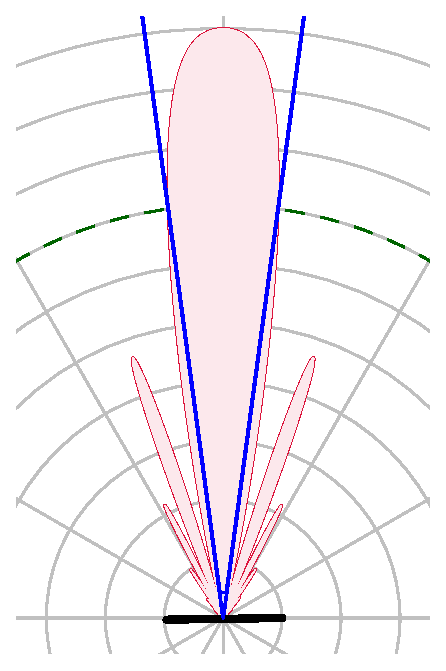
\includegraphics[scale=0.6,trim={0.46 0.072 0.46
	1.03},clip]{Chap2/fig/directivity.eps}
	\caption{Farfield beam shape and its \textit{beamwidth} (in blue).}
	\label{fig:beamwidth}
\end{figure}

On the other hand, there are hydrophone arrays that can infer the sound
direction by relating the spacing between the transducers with the signal
difference received by each of them \cite{bearing}.




\subsection{Available Models}
\label{ss:avaible_models}
 
\cite{sonars:16} % tipos de sonar

\section{Simulation}

Works on \textit{computacional ocean
acoustics}, the subfield of knowledge that explores the algorithms that model
the ocean as an acoustic medium, are well documented by
\citet{Etter2013}. Most of these works focus on very long range simulations,
with its most important features been the ocean floor and sub-bottom region.

This work aim to reconstruct and simulate near-range partially closed
environments, as those created by humans. The motivation for such a choice comes
from hydroeletrict power plant water intake, it is a corridor-like environment
with possible obstacles on the bottom. This kind of envirnoment is not well
covered on the underwater acoustics literature, as such, some of the simulations
techniques are borrowed from the closelly related are of \textit{room acoustics}.

When constructing a simulation one has to consider the tradeoff between
simplicity/perfomance/accuracy. There are several possible techniques with
different applications and assumptions, this chapter will cover the most
relevant ones and further explore \textit{ray theory}, which has been used for
the simulation presented here.

\subsection{Techniques Overview}

The idea behind sound simulation techniques is to solve the wave
equation (eq. \ref{eq:wave}) considering all the physical interfaces as boundary
conditions. The equation, however, cannot be analitically solved due to common
present discontinuities caused by occlusions, specular highlights and other
facts that result in large variations of the field over small regions of the
domain of integration\cite{funkhouser2003survey}.

The single most important reason that differentiate the several approches
described here is the \textit{wave frequency}. For high-frequency (where sound
speed do not very much in a wavelength scale) geometric methods (ray theory) are
justifiable and preferable (in the computational sense) \cite{urick1979}. In the
case of low/mid - frequency or in the presence of caustics\footnote{A region of
high constructive interference that geometrically gives a point of infinity
rays convegence.} other wave methods (e.g. finite elements, normal modes,
parabolic approximation) should be applied.

Instead of using the full wave equation, the methods work with a simplified
time-independ version. It starts by assuming that the equation
\ref{eq:wave}:

\[ \nabla^2 p - \frac{1}{c^2_0}\frac{\partial^2}{\partial t^2} p = 0 \]

Has a solution on the format:

\[ p(x,t) = a(x)\vartheta(t) \]

So that:
\[ \frac{\partial}{\partial t}a = 0 \]
\[ \nabla^2 \vartheta = 0 \]

Substituting it back and rearanging terms, gives:

\[ \frac{\nabla^2 a}{a} = \frac{1}{c_0^2\vartheta} \frac{\partial^2}{\partial
t^2}\vartheta  \]

As the expressions on both sides vary indepently, ie. l.h.s. varies with space
$s$ and r.h.s. with time $t$, they must be constant. As a matter of ajusting the
equation to fit its stantard parametrization, this constant is chosen to be
$-k^2$, then:

\[ \frac{\nabla^2 a}{a} = -k^2  \]
\[ \frac{1}{c_0^2\vartheta} \frac{d^2}{dt^2}\vartheta = -k^2  \]

Or

\begin{equation}
\label{eq:helmholtz}
(\nabla^2 -k^2)a = 0 
\end{equation}

\[ (\frac{d^2}{dt^2} + (kc_0)^2)\vartheta = 0  \]

With the apropriate definition of $\omega \equiv kc_0 $ the last equation,
becomes:

\begin{equation}
(\frac{d^2}{dt^2} + \omega^2)\vartheta = 0
\end{equation}

Equation \ref{eq:helmholtz} is known as the (homogeneous) \textit{Helmholtz
equation} and describe the time-independ part of the wave propagation. The
values of $k$ and $\omega$ can be phisically interpreted as the spatial and
tempral angular frequency of the wave. As the wave equation is a linear
equation superposition applies, it is resoanble to take into consideration
one wave frequency at a time and superpose all these harmonics by Fourier
synthesis\cite{Lefebvre}.



\subsubsection{FEM - Finite Element Method}\cite{funkhouser2003survey}
\subsubsection{Ray theory} \cite{torres2007modeling} \cite{danesh2013real}
\subsubsection{Normal modes} \cite{Etter2013}(?)
\subsubsection{Parabolic approximation} \cite{LURTON}

\subsection{Ray Theory}
\subsection{3D Enviroment Specifics}
\subsection{Results}

\section{Environment}

Extensive literature have been written on ocean environment, from modeling its
behaviour to measuring its properties. Different simulation techniques have also
been explored\cite{Etter2013}. The modeling presented here, althouth simple,
completely suits the needs of a ray tracing technique, presented on section
\ref{ss:raytheory}.

\subsection{Modeling}
\label{ss:modeling}
Borrowed from computer graphics, the modeling properties of a scene objectes
are the same for light and sound (given the high frequency limit for which ray
theory is applicable). Two distinct factors are modeled, one is geometric,
which defines the shape of the object, the other is acoustic, expressing how
does it interact with sound.

For the geometric part, two basic functions have to be provided: \textbf{intersection}
and \textbf{normal}. \textbf{Intersection} takes a ray, defined by a origin point and a
direction, and outputs the distance to the first intersection point with the
object. If no intersection point is found, the distance is defined to be
infinity. \textbf{Normal} receives a point on the surface of the object and
return the normal vector at such a point. Algorithm \ref{alg:rectangle}
exemplifies the \textbf{intersection} for a rectangle, the rays origin
$\mathbf{O}$ and direction $\mathbf{D}$ are matrix with the concatenated
information of all those whose intersection ought to be calculated.

\begin{algorithm}
\caption{Intersection for Rectangle}
\label{alg:rectangle}
\begin{algorithmic}
\Function{Intersection}{$\mathbf{O},\mathbf{D}$}\Comment{$\mathbf{O}$
is ray origin, $\mathbf{D}$ is direction} 

\State $\Delta \gets center -
\mathbf{O}$ \Comment{$center$ is the rectangle center}

\State $n \gets \nicefrac{\vec{s_1} \times  \vec{s_1}}{\norm{\vec{s_1} \times  \vec{s_1}}}$
\Comment{$\vec{s_1}$ and $\vec{s_1}$ are the rectangle's half-sides} 
\State $T \gets \left[ \vec{s_0} ~ \vec{s_1} \right]^\dagger$
\Comment{$^\dagger$ is pseudoinverse}
\State $d \gets \nicefrac{\Delta \cdot n}{\mathbf{D} \cdot n}$
\Comment{distance to intersection point}
\State $P \gets \mathbf{D}d - \Delta$
\Comment{$P$ are the intersection with the rectangle's plane}
\State $R \gets T \cdot P$
\Comment{$R$ are the intersection described on $\left[ \vec{s_0} ~ \vec{s_1}
\right]$ basis}

\ForAll{$i \in \left[0,\ldots,\text{size}(d)\right)$}
\If {$d_i < 0$ or $|R_{i,0}|>1$ or $|R_{i,1}|>1$}
\State $d_i \gets \infty$
\Comment{Check ray direction and if hit within rectangle}
\EndIf  
\EndFor


\State \textbf{return} $d$

\EndFunction
\end{algorithmic}
\end{algorithm}

Any surface can be approximated by triagulation and have these functions more
easily defined, but it is interesting to directly define for some geometric
primitives. Plane, rectangle, sphere and cylinder were developed for this work.

Two environments were constructed using these four geometric primitives. One
box-like for the reconstruction part of this thesis, which is simple enough to
study the properties of the mapping. Another, more complex and inspired on a
water entrance of a hydroeletric powerplant, that exibits a richer sonar
response with sound multipath and directional gain playing a more imporntant
role.

For the \textbf{box-like structure}, five planes were used thus determining a
semi-infinite box with 8 meters width, 10 meters length and the bottom 3 meters
from the origin. All planes are defined by a point and its normal vector.

\begin{table}[ht]
\centering
\begin{tabular}{lcc}
Plane Number & Point & Normal Vector \\
\hline
0 & $( 0, 4, 0)$ & $( 0,-1, 0)$  \\
1 & $( 0,-4, 0)$ & $( 0, 1, 0)$  \\
2 & $( 5, 0, 0)$ & $(-1, 0, 0)$  \\
3 & $(-5, 0, 0)$ & $( 1, 0, 0)$  \\
4 & $( 0, 0,-3)$ & $( 0, 0, 1)$  \\
\end{tabular}
\caption{Five planes defining box-like environment walls.}
\end{table}

The more \textbf{complex scene} is composed of 5 rectangles, 2 planes and a sphere
representing, respectively, 5 contrete walls, river floor and still surface
water and a half-spherical montain of sediments. Rectangles are defined by a
central point and two perpendicular vectors, the half sides, and spheres by a
center and radius.

\subsection{Characterization}
\label{ss:characterization}

Instead of defining a full BRDF (explained on section
\ref{sss:rays}), three parameters are considered: \textbf{diffusion coefficient},
\textbf{specular coefficient} and \textbf{shininess}. All three parameters may
change at every point on the surface of an object, thus defining a texture, but
for the sake of simplicity only constant values over the surface were
considered.

The \textbf{diffusion coefficient} and \textbf{specular coefficient} are,
respectively, fractions of incident energy over a surface patch that reflects
diffusely (as a lambertian reflector) and specularly. Reflections near
specularity are weighed as Phong reflection for a less unrealiscaly abrupt
change in reflection intensity. The \textbf{shininess} is the Phong parameter.
These concepts are described in section \ref{sss:rays}.

The actual values used came from a collection of sources in addition to
experimentation and tacit knowledge (from previous sonar use), as these are
difficult information to find in the literature.

For concrete, \citet{chirp} studies the \textbf{reflection coefficient}, sum of
\textbf{diffusion coefficient} and \textbf{specular coefficient}, to
characterize the concrete's quality following earlier measurements of
\citet{leslie1949ultrasonic}. The table provided on the article can be used in
the other direction, to simulate such a concrete quality. The individual values of \textbf{diffusion coefficient} and \textbf{specular coefficient} still
have to be determined and come from a educated guess based on considerations of
smooth by \citet{Etter2013}, which claims that most of the energy goes as
specular reflection for smooth surfaces. For
simulation purposes it has been consided values between 80\% to 95\% of the reflected energy to be specular.

\begin{table}[ht]
\centering
\begin{tabular}{rc}
Quality Of Concrete & Reflection Coefficient \\
\hline
Very good & $0.76$ or above  \\
Good & $0.69$-$0.74$  \\
Questionable & $0.62$-$0.69$  \\
Poor & $0.48$-$0.62$  \\
Very Poor & $0.48$ or less  \\
\end{tabular}
\caption{Quality of Concrete and Reflection Coefficient.
(\citet{chirp,leslie1949ultrasonic})}
\end{table}

\citet{Etter2013}, also, provides equations relating wind speed with water
surface reflection coeffiecient, which varies according to its roughness caused
by the wind. For a still water there is amost no transmitted energy and all
reflected energy is specular. For other materials, estimated values come from
models as the one provided by \citet{miller2015real} on
figure\ref{fig:materials}.

\begin{figure}[h]
	\centering
	\includegraphics[width=0.8\textwidth]{Chap2/fig/materials}
	\caption{Materials reflective characteristics from \citet{miller2015real}.}
	\label{fig:materials}
\end{figure}


%\subsection{3D Enviroment Specifics}
\section{Implementation}

\subsection{Algorithm}
\label{ss:algorithm}

The simulation follows the ray tracing technique outlined by
~\citet{bell1997simulation} for side scan sonar, but applies it to a forward
looking sonar imaging sonar (Section \ref{ss:avaible_models}). It also uses a
noising adding step as suggested by~\citet{coiras2009gpu} with statistics
provided by~\citet{maussang2007mean}.
No movement induced distortion was considered, some approaches to add this
feature is available in~\citet{bell1999techniques,borawski2005sonar}. Also,
spreading and absorption losses are ignored, assuming they are compensated by
TVG (see Section \ref{sss:tvg}).

Sonar parameters follow a Tritech's Micron sonar~\cite{micronsonar}
information as output power, dynamic gain, beam step and sensibility were found
on official Tritech's documentation~\cite{micronsonar,micronmodem}. The directional
gain was measured by the National Physical Laboratory, UK.

Simulation's output is, just as on the sonar, a sequence of arrays with values
between 0 and 255. Each element of the sequence is a bearing, direction of the
emitted sound pulse, and the array's components are the bins' values, sound
intensity received at some range of distances (calculated from echo delay).

\begin{figure}[h]
	\centering
	\includegraphics[scale=1.,clip]{Chap2/fig/sonarresponse.eps}
	\caption{Example of an array for a bearing direction. Actual arrays are
	longer, depending on resolution.}
	\label{fig:bins}
\end{figure}

The algorithm implementation uses the programming language Python with the
mathematical library NumPy, specially for efficient linear algebra. Most of the
treatment uses linear algebra to treat batch of rays at once.

\begin{figure}[ht]
    \centering
    \subfloat[Sonar Loop]{{\includegraphics[width=65mm]{Chap2/fig/sonarflow}}}%
    \hfill
    \subfloat[RayTracer]{{\includegraphics[width=85mm]{Chap2/fig/raytraceflow}}}%
    \caption{Overview of the simulation algorithm.}%
    \label{fig:algorithm}%
\end{figure}

Flowchart of Figure \ref{fig:algorithm} describes the simulator logic. It starts
by computing ray directions spread over a sphere centered at the sonar with
uniform density, otherwise it would bias the ray trace. Not all directions are
actually computed because some directions have very low gain, so rays in these directions
have almost no energy, they can be discarded. To compute such a uniformly
distributed directions apply transformation described by algorithm
\ref{alg:urays} for $[-\alpha,\alpha]$ and $[-\beta,\beta]$ the vertical and
horizontal angular span, respectively, and $N$ the desired number of rays.
Results in Section \ref{ss:results} use $\alpha = 30^o$ and $\beta = 3^o$,
approximatly the values for which Micron cannot detect the echo. 


\begin{algorithm}
\caption{Rays Uniform Direction}
\label{alg:urays}
\begin{algorithmic}
\Procedure{Uniform Direction}{$\alpha,\beta,N$}

\State $\dif\theta \gets 2\cos(\nicefrac{\pi}{2}-\alpha)$
\State $\dif\phi \gets 2\beta $
\State $\rho \gets \sqrt{\frac{N}{\dif\phi\cdot\dif\theta}}$ \Comment{Estimated
density}
\State $N_\theta \gets \lceil\rho\cdot\dif\theta\rceil$
\State $N_\phi \gets \lceil\rho\cdot\dif\phi\rceil$
\Comment{$U(\coord{x})$ generates $\coord{x}$ uniform samples over $[0,1]$}
\State $\theta \gets \arccos(\dif\theta\cdot (2U(N_\theta)-1))$ 
\State $\phi \gets \dif\phi\cdot (2U(N_\phi)-1)$

\ForAll{$(\theta_i,\phi_i) \in \theta\times\phi$}
\State $x_i \gets \sin(\theta_i)\cos(\phi_i)$
\State $y_i \gets \sin(\theta_i)\sin(\phi_i)$
\State $z_i \gets \cos(\theta_i)$
\State $v_i \gets (x_i,y_i,z_i)$
\EndFor

\State \textbf{return} $v$
\EndProcedure
\end{algorithmic}
\end{algorithm}

The sonar bearing pace is adjustable and, following Tritech's Micron
configuration, it was set to $1.8^o$, thus, doing a complete scan on $200$ steps. For each step, ray
directions are changed (by a rotation) to match new bearing. Received gain is
calculated w.r.t. the front direction (bearing), as the bearing changes the gain
is automatically updated. Rays always carry 2 information: its actual
intensity (disregarding distance traveled decay) and its total traveled length.

A new bearing position invoke ray tracer algorithm. It begins by calling
the \textbf{intersection} function (described in Section \ref{ss:modeling}) for
each object in the scene, passing all rays as argument. Then it loops again on every
object, but now only focus on the rays that have the object as first hit, and
compute the backscattering to the sonar. Backscattering strength calculation use
Lambert and Phong scatterings as described in Section \ref{sss:rays} and material
parameters listed in Section \ref{ss:characterization}. This strength is addad
to a bin (see Figure \ref{fig:bins}) whose position is calculated as half the full
distance traveled by the ray (including previous reflections) plus a small
gaussian noise. It proceeds to calculate reflection if the number of computed
reflection for the ray does not exceed a maximum value (set to 5). Reflections
are simple linear transformations that depends on the surface's normal, obtained
via \textbf{normal} function (Section \ref{ss:modeling}). The algorithm, then,
calls itself for the reflected rays, recursively.

\begin{figure}
	\centering
	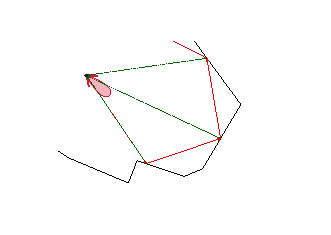
\includegraphics[scale=2.5, trim={20 20 20 20}, clip]{Chap2/fig/method.pdf}
	\caption{Ray Tracing: Red lines are specular reflections, green lines are diffuse backscattering.}
	\label{fig:methodtrace}
\end{figure}

After the whole scan is computed, bin values are normalized to $[0,\ldots,255]$
(again according to Tritech's Micron configuration ). Upon these values, an
additional Weibull's distributed noise is applied~\cite{maussang2007mean}.

\subsection{Results}
\label{ss:results}

For both environments described in Section \ref{ss:modeling}, several sonar
positions were simulated. The absolute position and orientation were chosen, but
the bearing w.r.t. the environment was a random value.

Polar plots displayed here is the expected visualization, without noise
filtering, when the sonar uses 500 bins of resolution with a 12 meters range.
Each polar pixel has a $3^o$ arc length, but, as the bearing step is $1.8^o$,
they overlap while being rendered.

\subsubsection{Box-like Environment}
The half-infinity box-like structure is depicted on figure
\ref{fig:box_simul}. Axis aligned sonar orientation on figures
\ref{fig:box_axis_center} and \ref{fig:box_axis_offcenter} make clear its
rectangular cross section, while its half-infinity characteristic is visible on
perpendicular oriented scans, figures \ref{fig:box_perp_center} and
\ref{fig:box_perp_offcenter}.


\begin{figure}[ht]
    \centering \subfloat[Position $(0,0,0)$ | Orientation
    $(1,0,0)$]{{\label{fig:box_perp_center}\includegraphics[width=75mm]{Chap2/fig/main_script__4_13_57_42_0,0,0_1,0,0f2}}}%
    \hfill \subfloat[Position $(4,1,0)$ | Orientation
    $(0,1,0)$]{{\label{fig:box_perp_offcenter}\includegraphics[width=75mm]{Chap2/fig/main_script__4_14_12_04_4,1,0_0,1,0f2}}}%
    \\
    \subfloat[Position $(0,0,0)$ | Orientation
    $(0,0,1)$]{{\label{fig:box_axis_center}\includegraphics[width=75mm]{Chap2/fig/main_script__4_14_14_06_0,0,0_0,0,1f2}}}%
    \hfill \subfloat[Position $(0,3,0)$ | Orientation
    $(0,0,1)$]{{\label{fig:box_axis_offcenter}\includegraphics[width=75mm]{Chap2/fig/main_script__4_14_18_20_0,3,0_0,0,1f2}}}%
    \caption{Sonar simulation for the box-like scene.}%
    \label{fig:box_simul}%
\end{figure}

\subsubsection{Complex Environment}

Figure \ref{fig:jirau_simul} shows the more complex structure from four view
points. Images \ref{fig:complex_inner_mid} and \ref{fig:complex_inner_low} are scans from between walls of the indent. Figure
\ref{fig:complex_out_mid} is cross sectional view of the indent and figure
\ref{fig:complex_out_low} is a scan from the same position, but with different
orientation, making the hemisphere at the bottom more noticeable.

\begin{figure}[ht]
    \centering \subfloat[Position $(0,0,0)$ | Orientation
    $(1,0,0)$]{{\label{fig:complex_inner_mid}\includegraphics[width=75mm]{Chap2/fig/main_script__4_02_09_57_0,0,0_1,0,0f2}}}%
    \hfill \subfloat[Position $(0,0,6)$ | Orientation
    $(1,0,0)$]{{\label{fig:complex_inner_low}\includegraphics[width=75mm]{Chap2/fig/main_script__4_02_10_19_0,0,6_1,0,0f2}}}%
    \\
    \subfloat[Position $(-5,0,12)$ | Orientation
    $(0,1,0)$]{{\label{fig:complex_out_low}\includegraphics[width=75mm]{Chap2/fig/main_script__4_02_16_13_-5,0,12_0,1,0f2}}}%
    \hfill \subfloat[Position $(-5,0,12)$ | Orientation
    $(0,0,1)$]{{\label{fig:complex_out_mid}\includegraphics[width=75mm]{Chap2/fig/main_script__4_02_21_25_-5,0,12_0,0,1f2}}}%
    \caption{Sonar simulation for the complex scene.}%
    \label{fig:jirau_simul}%
\end{figure}

Both environemnts reveal interesting features of a sonar scan, but they tend to
be more pronounced on the complex environmnt. Figures
\ref{fig:complex_inner_low}, \ref{fig:complex_out_mid} and
\ref{fig:box_perp_offcenter} present clear signal of multipath. Another
interesting feature is the halo on the background of figures
\ref{fig:complex_inner_mid} and \ref{fig:complex_inner_low} caused by a
trade-off between the sonar directional gain and the low backscattering at
shallow angles.

\chapter{Mathematical Preliminaries}

\epigraph{"Obvious" is the most dangerous word in mathematics.}{\textit{Eric Temple
Bell}, 1938}

Some of the more advanced mathematical tools\footnote{As judged by the autor
from the perspective of a graduated student.} used on the development of this
thesis are presented here.
Other knowledges, as basic linear algebra, statistics and analysis, are take as
granted.


\section{Hilbert Space}
\label{s:hilbert}
A Hilbert Space is a complete inner product space \cite{HS-YN:11}. It is a
complete metric space with respect to the metric induced by its inner product
(which in turn can be thought indirectly by its induced norm). A nice picture
is as a generalization of the Euclidean space. Which means intuition works well,
in contrast with the broader concept of Banach Spaces, a complete normed space,
where the infinite dimensional case can be quite different from what one would
expect\footnote{Banach Space are complete metric spaces where the metric does
not come necessarily from a inner product. (See \citet{HS-HJNB:00})}.

An inner product space\cite{HS-HJNB:00} is a (possibly infinite dimensional)
vector space $V$ over $\mathbb{C}$ (or $\mathbb{R}$ by restriction ), together
with a map (called the \textbf{inner product}):

\[  \langle\cdot,\cdot\rangle_{\scriptscriptstyle V}: V \times V \to \mathbb{C}
\]

Satisfying the following properties, for all $x,y,z \in V$ and all $\mu, \lambda
\in \mathbb{C}$:

\begin{enumerate}[I]
  \item \(  \langle x,\lambda y + \mu z  \rangle_{\scriptscriptstyle V} = \lambda\langle	
  x,y\rangle_ {\scriptscriptstyle V} + \mu \langle x,z \rangle_{\scriptscriptstyle V} \) (linear in the second argument)
  \item \( \langle x,y \rangle_{\scriptscriptstyle V} = \overline{\langle y,x \rangle_{\scriptscriptstyle V} } \)
  (Hermitian symmetric)
  \item  \( \langle x,x \rangle_{\scriptscriptstyle V} \geq 0 \) and \( \langle x,x \rangle_{\scriptscriptstyle V} = 0
  \Leftrightarrow x = 0 \) (positive definite)
\end{enumerate}

A classical example of a inner product is the Euclidean dot product.

Another important example is the inner product defined on the space C$[a,b]$ of
complex (or real) valued continuous functions on the interval $[a,b]$, defined,
for every $f$ and $g$ in C$[a,b]$ as:

\begin{equation}\label{eq::func_inner}
  \langle f,g\rangle_{\scriptscriptstyle \text{C}[a,b]} = \int_a^b
  f(x)\overline{g(x)} \mathrm{d}x
\end{equation}

On any Hilbert Space $\hs$ the norm induced by the inner product is:

\begin{equation}
  \hnorm{x} = \sqrt{ \hip{x}{x} }
\end{equation}

where $x \in \hs$. And the subsequent metric is defined as:

\begin{equation}\label{eq::norm_metric}
  d_{_\hs}(x,y) = \hnorm{ x - y }
\end{equation}

for any $x,y \in \hs$.

A vector space endowed with a inner product is a \textit{inner product space}
(aka. pre-Hilbert space). For it to be a Hilbert Space it also has to be complete
with respect to the above metric. Completeness means that any Cauchy sequence
converges in this space (which provides a suitable framework to apply the tools
of calculus). A Cauchy sequence is a sequence where every term becomes
arbitrarily close to each other as the sequence progress (not only to term
right next to it). It can be formalized as the sequence
$x_1$,$x_2$,$x_3$,$\ldots$ on a metric space (with a metric $d( \cdot ,\cdot)$)
where:


\[ \forall \epsilon \in \mathbb{R}^+, ~\exists N \in \mathbb{Z}^+, ~\forall
n,m>N \Longrightarrow ~d(x_n,x_m)<\epsilon
\]

On a pre-Hilbert space, the metric is given by equation \ref{eq::norm_metric}.
If a metric space $M$ is complete, then every Cauchy sequence
($x_1$,$x_2$,$x_3$,$\ldots$) converges in that space:

\[ \exists x \in M, \forall \epsilon \in \mathbb{R}^+, ~\exists N \in \mathbb{Z}^+, ~\forall
n>N \Longrightarrow ~d(x_n,x)<\epsilon
\]
So,
\[ x = \lim_{n\to\infty} x_n \]

A complete metric space can be obtained from a pre-Hilbert space, by completion,
in the same way that $\mathbb{Q}$ is ``completed'' to make $\mathbb{R}$.
Although completeness is a technicality, it is easy to find examples of
pre-Hilbert spaces that lacks this property. The space of continuous functions
C$[a,b]$ with the inner product defined on \ref{eq::func_inner} gives an example
of pre-Hilbert space that is not complete. For it to be a Hilbert space, the
space have to be extend to include some discontinuous functions, as in the larger
set of Lebesgue mensurable\footnote{The Lebesgue mensurability of a, bounded
with compact support, function is a highly technical exigence and the existence
of a bounded non-Lebesgue mensurable set (which allow the construction of such a
function) is dependent on the axiomatic choice of the underlying set theory - it
can only be proven with the adition of the \textit{choice axiom} to the
ZF (Zermelo-Fraenkel) set of axioms (ZFC). } functions that are square
integrable (with the Lebesgue integral).

Some examples of Hilbert space are:

\begin{itemize}
  \item Any finite dimensional vector space over the field $\mathbb{R}$ or
  $\mathbb{C}$ with the standard dot product.
  \item The space $\ell^2$ of square-summable sequences of complex numbers, i.e.
  $(c_1,c_2,c_3,\ldots)$ with $c_i \in \mathbb{C}$ and $\sum_{i=1}^\infty |c_i|^2 <
  \infty$, is a Hilbert space with the inner product defined as: Given two
  sequences $x=(x_1,x_2,x_3,\ldots)$ and $y=(y_1,y_2,y_3,\ldots)$, define $\langle x,y
  \rangle_{\scriptscriptstyle \ell^2} = \sum_{i=1}^\infty x_i \bar{y_i}$.
  \item Fourier series can be seen as the representation of a square-integrable
  function on the interval $[0,1]$ (member of $L^2[0,1]$) on the orthogonal
  basis $\{\mathrm{e}^{2\pi i n \theta} : n \in \mathbb{Z}\}$ with the
  inner product given by \ref{eq::func_inner}.
\end{itemize}


\section{RKHS - Reproducing Kernel Hilbert Space}

A \textit{Reproducing Kernel Hilbert Space}, RKHS for short, is a special kind
of Hibert Space of functions. In a RKHS, closeness in the sense of the metric is
actual pontwise proximity. That is to say, if two real-valued functions $f$ and
$g$ of a (non-empty) set $\mathcal{X}$ belong to a RKHS $\hs$ ($f,g \in \hs
\subset \mathbb{R}^\mathcal{X}$), then whenever $\hnorm{f-g}$ is small so is
$\norm{f(x)-g(x)}$ for all $x \in \mathcal{X}$\cite{berlinet2011reproducing}.

A more formal and useful characterization of a RKHS is consequece of studying
linear operators on Hibert Spaces. The evaluation functional \(\delta_x: \hs \to
\mathbb{R}\), \(\delta_x: f \to f(x)\) is easily seen as such: given \(f,g \in
\hs\) and \(a,b \in \mathbb{R}\), \(\delta_x(af+ag)= (af+ag)(x) = af(x)+ag(x) =
a\delta_x(f)+b\delta_x(g)\). When the evaluation functional is continuous on
$\hs$, $\hs$ is said to be a RKHS.

Riesz representation theorem is an extension, for Hibert Spaces, of the
classical isomorphism between a finite vector space $\mathcal{V}$ and its dual
$\mathcal{V}^*$, the space of linear functions on $\mathcal{V}$. It states that
for every element $\phi \in \hs^*$, where $\hs^*$ is the space
\textit{continuous} linear functionals from $\hs$ into $\mathbb{R}$ (dual
space), there exist a unique $y_\phi \in \hs$, defined by:
\begin{equation}
\phi(x)= \hip{x}{y_\phi}
\end{equation}

 As consequece

\citet{berlinet2011reproducing} -  Quase tudo sobre RKHS

\section{Probabilistic Regression}

Probabilistic regression is similar to classification, both infer properties of
a sample based on previous information. However, instead of giving a definite
answer for which class an element belongs, probabilistic regression gives the
probability for such a classification~\cite{jaakkola1999probabilistic}. More
formally, a training set is a sequence of $n$ pairs
$\{(x_i,y_i)|~i=1,\ldots,n\}$, where $x_i$ and $y_i$ are samples drawn from
random variables $X$ and $Y$, respectively, with joint probability distribution
$\Pr(X,Y)$~\cite{friedman2001elements}. From this training set, a conditioning
probability $\Pr(Y|X=x)$ has to be estimated.

The special case where $Y$ is a Bernoulli random variable, i.e. a binary
variable, is called binary regression. It is the single most important
regression for mapping, as such, no other kind is explored in this thesis. 

\subsection{Binary Logistic Regression} 
\label{ss:blr}
A binary regression dependent variable $Y\in\{-1,1\}$
(or some set of equal cardinality like $\{0,1\}$) has two
possible estimations that are related by $\Pr(Y=1|X=x)+\Pr(Y=-1|X=x)=1$. As
such, the conditional probability can be denoted
\begin{equation*}
p(x) = \Pr(Y=1|X=x) 
\end{equation*}

The probability for $Y=-1$ can be recovered from $P(Y=-1|X=x)=1-p(x)$. The
linear logistic model~\cite{ramos2016hilbert} $p(x;\coord{w})$ for
$x\in\mathbb{R}^d$, with $\coord{w}\in\mathbb{R}^d$ as explicit parameter:

\begin{equation}
\label{eq:std_linear_logistic}
p(x;\coord{w}) = \frac{1}{1+\exp(-\coord{w}\cdot x)}
\end{equation}

The rationale behind the model is that the function
$(1+\exp(-\alpha))^{-1}$ is a bijection
$\mathbb{R}\to(0,1)$~\cite{friedman2001elements}. Ensuring that the model is a
probabilistic distribution.

The classical regression theory requires a loss function $\mathscr{C}$ and
minimizes an empirical risk over some space of functions
$R[f]=\mathbb{E}(\mathscr{C}(X,Y,f(X)))$~\cite{jaakkola1999probabilistic},
where $\mathbb{E}(\parm)$ is the expected value.
The estimation of $f$ from samples $(x_i,y_i)$ uses a regularized version:
\begin{equation}
\label{eq:regularized_estimator}
R_{\text{reg}}[f] =
\frac{1}{n}\sum_{i=1}^n\mathscr{C}(x_i,y_i,f(x_i))+\lambda\mathcal{S}[f]\,,
\end{equation}
%
where $\lambda>0$ and $\mathcal{S}[\parm]$ stabilization (regularization) term,
as the minimization problem is typically
ill-posed~\cite{jaakkola1999probabilistic}. On normed spaces usually
$\mathcal{S}[f]=g(\norm{f})$, where $g(\parm)$ is a monotonically increasing
function. With proper adjustment of $\lambda$, the $\nicefrac{1}{n}$ factor
might be ignored without changing the minimizing function.
The loss function $\mathscr{C}$ is problem dependent and for binary regression a
typical negative log likehood (NLL\abbrev{NLL}{Negative Log Likehood}) is used
\begin{equation}
\label{eq:general_nll}
\mathscr{C}(x,y,p(x)) = - \log \Pr(Y=y|X=x) = 
\begin{cases} 
      - \log p(x) & y=1 \\
      - \log (1-p(x)) & y=-1
   \end{cases}
\end{equation}

For a linear logistic model, one uses (\ref{eq:std_linear_logistic}) on
(\ref{eq:general_nll}) and substitutes back into
(\ref{eq:regularized_estimator}).
Thus the regularized negative log likehood empirical risk simplifies to a $d$
dimensional minimization:
\begin{equation}
\label{eq:classicnll}
\text{NLL}_{\text{reg}}(\coord{w}) =  \sum_{i=1}^n \log(1+\exp(-y_i
\coord{w}\cdot x_i)) +\lambda\mathcal{S}(\coord{w})\,.
\end{equation}


Reasonable choices for $\mathcal{S}(\parm)$
are the $\ell_1$ norm (LASSO)
$\mathcal{S}(\coord{w})=\norm{\coord{w}}_1$
or elastic net, a combination of $\ell_1$ (LASSO) and
squared $\ell_2$ norms (ridge),
$\mathcal{S}(\coord{w})=\alpha_1\norm{\coord{w}}_1
+\alpha_2\norm{\coord{w}}_2^2$, where
$\alpha_1+\alpha_2=1$, $\alpha_1,\alpha_2\in[0,1]$~\cite{hastie2015statistical}.


Although it is an applicable setting for simple situations, it is not expected
to perform well for classification/regression of point on a 3D environment as
$x\in\mathbb{R}^3$ and $\coord{w}\in\mathbb{R}^3$. The three real parameters,
encoded by $\coord{w}$, is not enough to capture all the complexities of the
environment. To keep the simplicity provided by the linear model and still be
suitable for a three dimensional map, an alternative is to increase
dimensionality using Hilbert Spaces.

\subsection{Regression on Hilbert Spaces}
\label{ss:reg_hs}
Samples defined on a low dimensional space $\mathcal{X}$, e.g. $\mathbb{R}^3$,
can be raised to a high (possible infinite) dimensional space using a feature
map $\varphi:\mathcal{X}\to\hs$, where $\hs$ is hilbert space. This allow
linear models to express more generic functions $f(x) =
\hip{\coord{w}}{\varphi(x)}$ with $\coord{w}\in\hs$, such a space of functions
$f(x)$ is the actual RKHS with kernel define as in equation
(\ref{eq:feature_kernel}).

The linear logistic model from equation (\ref{eq:std_linear_logistic}) lifted to
the Hilbert Space $\hs$ is
\begin{equation}
\label{eq:hslogistic}
p(x;\coord{w}) = \frac{1}{1+\exp(-\hip{\coord{w}}{\varphi(x)})}
\end{equation}

Thus, equation (\ref{eq:classicnll}) for log likehood empirical risk
becomes\footnote{With appropriate adjustment of $\lambda$'s value,i.e.
$\lambda=n\lambda_0$, the usual average $\nicefrac{1}{n}$ for the summation can
be dropped, as it keeps the same minimizer value of $\coord{w}$.}
\begin{equation}
\label{eq:hsnll}
\text{NLL}_{\text{reg}}(\coord{w}) =  \sum_{i=1}^n \log(1+\exp(-y_i
\hip{\coord{w}}{\varphi(x_i)})) +\lambda\mathcal{S}(\coord{w})
\end{equation}

In practice, one chooses a kernel $K(x,y)$ with desired properties and
find finite dimensional approximate features $\hat\varphi(x)$, such that
$K(x,y)=\hip{\varphi(x)}{\varphi(y)}\approx\hat\varphi(x)\cdot\hat\varphi(y)$.
Non kernel specific methods for finding approximate features include sampling
the Fourier transform of shift invariant kernels~\cite{rahimi2007random}, i.e.
$K(x,y)=k(x-y)=k(\delta)$, and Nystr\"om method that projects the Gram matrix
$\mathbf{G}_{ij}=K(x_i,x_j)$ of the sample points $\{x_i\}$ into some subset of
these points and use this projection to approximate the feature
maps~\cite{williams2000using}.

\backmatter
\bibliographystyle{formating/coppe-unsrt}
\bibliography{biblio}

\end{document}
